\documentclass[12pt, letterpaper, twoside]{article}
\usepackage[utf8]{inputenc}

\usepackage{geometry}
\usepackage{algorithm}
\usepackage{algpseudocode}
\usepackage[backend=bibtex,style=verbose-trad2]{biblatex}
\usepackage{amssymb}
\usepackage{amsmath}

% \setlength{\parindent}{4em}
\setlength{\parskip}{1em}
\bibliography{citation-13218946.bib}

\title{Solucionando el problema de la mochila en el Modelo Sticker}
\author{Ernesto Mancebo}
\date{Febrero 2020}

% \tikzset{
%     pics/realline/.style 2 args = {
%         code = {
%             \draw [thick] (0,0) -- (6,0) node [right=2mm] {$$mathbb{R}};
%             \fill[black] (1,0) circle (1mm) node[abobe=2mm] {$#1$}
%                          (3,0) circle (1mm) node[abobe=2mm] {$#2$}
%                          (6,0) circle (1mm) node[abobe=2mm] {$V_4$};
%             \foreach \i [count=\j] in {0,0.5,1,1.5,3,4.5,6}
%                 \coordinate (-\j) at (i,0);
%         }
%     }
% }
\usepackage{tikz}
% \usetikzlibrary{positioning}

\tikzset{
  mynode/.style={fill,circle,inner sep=2pt,outer sep=0pt}
}


\begin{document}
    \maketitle
    \begin{abstract}
        Este documento tiene como objetivo la resolución de los problema \emph{suma de subconjuntos} y \emph{porblema de la mochila}, para éste último en sus versiones acotada y la no acotada, utilizando como apoyo para la resolución de ambos problemas las subrutinas \emph{ordenado por cardinalidad} y \emph{llenado en paralelo}.
    \end{abstract}

    \newpage
    \section{Introducción}
    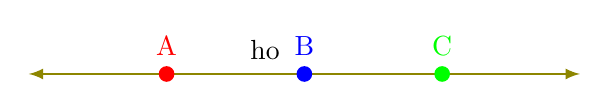
\begin{tikzpicture}
        \draw[olive,thick,latex-latex] (0,0) -- (7,0)
        node[pos=0.25,mynode,fill=red,label=above:\textcolor{red}{A}]{}
        node[pos=0.5,mynode,fill=blue,text=blue,label=above:\textcolor{blue}{B}]{}
        node[pos=0.75,mynode,fill=green,text=green,label=above:\textcolor{green}{C}]{};

        \node at (3,0.3) {ho};
    \end{tikzpicture}

    \section{Modelo Sticker}
    El Modelo Sticker es un modelo de computación inpirado en cadenas de ADN propuesto por Sam Roweis \textcolor{red}{\cite{article}}, donde tal modelo se basa en procedimientos de filtrado, con memoria de acceso aleatorio y una nueva manera de codificar la información. En ese mismo orden, se distingue de otros modelos computacionales por la manera en que codifica la información.

    \subsection{Conceptop de Cadena de Memoria}
    El eje central de este modelo son las cadenas de memoria, tales cadenas consisten en hebras simples de ADN del tipo $(n, k, m)$, tal que $n\geq k.m$, siendo $n$ la longitud de la cadena, $k$ las cantidad de subcadenas o regiones, y $m$ la longitud de cada subcadena.\textcolor{red}{ Las cadenas de memoria también se les conocen como moléculas y son representadas por sigma ($\sigma$)}. \\ \\
    En ese mismo orden de ideas, un sticker es asociado a una región en la cadena de memoria
    % TODO
    las operaciones realizadas sobre cada hebra o complejo de memoria asocia un sticker a una región $k$, transformando la cadena en una hebra doble \emph{parcial}, tal que en cada región donde haya un sticker complementándole se dice que está \emph{encendido}, mientras que la región donde se carezca de sticker se dice está \emph{apagado}. Tal abstracción binaria también se puede expresar de modo \emph{0/1}.
    % TODO

    \subsection{Concepto de Tubo}
    Dentro de este modelo, conocemos un tubo como un multiconjunto de complejos de memorias del mismo tipo. Tal concepto se puede representar como una matriz de complejos de memoria $\sigma$ del modo:
        $
        \left[
            \begin{array}{l}
                \sigma_0 \\
                \sigma_i \\
                \sigma_{i + 1} 
            \end{array}
        \right]
        $ \\
    En ese orden de ideas, las operaciones a principales dentro de este modelo son:
    \begin{itemize}
        \item \emph{mezclar}$(T_1,T_2)$: Retorna la unión de los dos tubos devolviendo un solo tubo el cual contiene cada complejo de memoria proveniente de ambos. También se nota como $(T_1\bigcup T_2)$.
        \item \emph{separar}$(T, i)$: Para un tubo $T$ y un $i$ tal que $(1 \leq i \leq n)$, siendo $n$ la cantidad de subcadenas para cada complejo de memoria, retorna un $+(T, i)$ y $-(T, i)$, de modo que el primer tubo contiene todos los complejos de memoria cuya región $i$ esté encendida (\emph{on} o $1$), mientras que la segunda lo contrario (\emph{off} o $0$).
        \item \emph{encender}$(T, i)$: Para un tubo $T$ y un $i$ tal que $(1 \leq i \leq n)$, siendo $n$ la cantidad de subcadenas para cada complejo de memoria, enciende la región $i$ de cada complejo de memoria asignando un $1$ u \emph{on}.
        \item \emph{apagar}$(T, i)$: Opuesto a \emph{encender}, asigna un $0$ u \emph{off}.
        \item \emph{leer}$(T)$: Dado un tubo $T\neq\emptyset$, lee su contenido.
    \end{itemize}
    \subsection{Concepto de Librería}
    Una librería dentro de este modelo es lo conocido como complejos de memoria de modo $(k,l)$ tal que, teniendo $k$ sub cadenas/regiones y las primeras $k - l$ subcadenas están \emph{on} u \emph{off}, en todas sus posibles combinaciones.

    \section{SubRutina Ordenado por Cardinalidad}
    Teniendo los siguientes elementos:
    \begin{itemize}
        \item $A = \{1,\cdots,p\}$
        \item $B = \{b_1,\cdots,b_s\} \subseteq A$ 
        \item $F = \{D_1,\cdots,D_t\} \subseteq P(A)$ 
    \end{itemize}
    Se busca ordenar $F$ con respecto a su cardinalidad en $B$, o en otras palabras, la cantidad de elementos que conincidan de manera $B\cap D_i$.
    Una vez teniendo claro el domino del problema planteado, el paper bajo estudio nos sugiere el implementar la codificación de cada familia de subconjuntos $F$, de forma que la familia mencionada sea una molécula $\sigma$ para el tubo $T_0$, codificando cada molécula de forma $T_0=\{\{\sigma:|\sigma|=p \land \exists j(\chi_{D_j}=\sigma)\}\}$; tal que $\chi_{D_j}$ es la función característica en $A$, siendo $(\chi_{D_j}(i) = 1$ si $i \in D_j$ de lo contrario $\chi_{D_j} = 0$ si $i \in A - D_j)$.
    Ya con las restrinciones definidas, se plantea en el paper una subrutina que en el paso \emph{i} se generen $i + 1$ tubos verificando la condición $\forall\sigma(\sigma\in T_j \rightarrow|\sigma\in\{b_1,\cdots,b_i\}|=j)$, leyéndose esta condición: sólo existirán moléculas $\sigma$ en $T_j$ cuya cantidad de regiones encendidas sean igual a $j$.
    \subsection{Algoritmo}
    En ese sentido, el paper ** sugiere el siguiente algoritmo:
    \begin{algorithm}
        \caption{Ordena los elementos en $T_0$ con respecto a los elementos de $B$ presentes en cada $\sigma$}
        \label{CardinalSort}
        \begin{algorithmic}[1]
            \Procedure{$Cardinal\_Sort$}{$T_0,B$}
            \For { $i=1$ to $s$ }
            \State $(T_0, T'_0) \leftarrow separar(T_0, b_i)$
            
            \For { $j=0$ to $i-1$ }
            \State {$(T'_{j+1},T''_j) \leftarrow separar(T_j,b_i)$}
            \State {$T_j \leftarrow mezclar(T'_j,T''_j)$}
            \EndFor
            \State {$T_i \leftarrow T'_i$}
            \EndFor
            \State Return $[T_0,...,T_s]$
            \EndProcedure
        \end{algorithmic}
    \end{algorithm}
    
    \subsection{Traza SubRutina Ordenado por Cardinalidad}
    A modo de ilustrar el comportamiendo y los conceptos empleados en el algoritmo concebido, tenemos:
    \begin{itemize}
        \item $A: \{0, 1, 2, 3, 4, 5, 6\}$
        \item $B: \{1, 2, 4\}$
        \item $F: \{\{2, 6\}, \{3\}, \{4\}, \{2, 4\}\}$
    \end{itemize}
    Observemos que los elementos que cumplen $B\cap D_j$ en $F$ son: $\{\{\textcolor{red}{2}, 6\}, \{3\}, \{\textcolor{red}{4}\}, \{\textcolor{red}{2, 4}\}\}$, cuyos elementos resaltados nos sugieren en qué posición del tubo de salida tras ser evaluados por \emph{Cardinal\_Sort}. Codificando $F$ para llevarlo a un tubo tendíamos: \\
    $
        \begin{bmatrix}
            0, 0, 1, 0, 0, 0, 1 \\
            0, 0, 0, 1, 0, 0, 0 \\
            0, 0, 0, 0, 1, 0, 0 \\
            0, 0, 1, 0, 1, 0, 0 \\
        \end{bmatrix}
    $
    Este $T_0$ codificando $F$ tras la ejecución de \emph{Cardinal\_Sort} tendremos: \\
    $
    \begin{bmatrix}
            T_0&: [[0, 0, 0, 1, 0, 0, 0]] \\
            T_1&: [[0, 0, 0, 0, 1, 0, 0], [0, 0, 1, 0, 0, 0, 1]] \\
            T_2&: [[0, 0, 1, 0, 1, 0, 0]] \\
            T_3&: [] \\
            T_4&: [] \\
            T_5&: [] \\
            T_6&: [] 
    \end{bmatrix}
    $
    Cumpliendo de esta manera la condición de $\forall\sigma(\sigma\in T_j \rightarrow|\sigma\in\{b_1,\cdots,b_i\}|=j)$.

    \subsection{Asunciones}
    Para usos posteriores dentro de este informe, podemos notar la llamada a \emph{Cardinal\_Sort} de modo:
    \begin{itemize}
        \item $Cardinal\_Sort(T_0)$ cuando $B=A$.
        \item $Cardinal\_Sort(T_0, l, k)$ cuando $B=\{l, l+1,\cdots,k\}$.
    \end{itemize}
    \section{SubRutina de Llenado}
    Una vez pensado en el concepto de codificar en $F$ las moléculas $\sigma$ tal que $B\cap D_i$, podemos considerar la idea de segmentar cada molécula $\sigma$ en $T_0$ en posibles regiones como:
    \begin{itemize}
        \item $(A\sigma )=\sigma (1)\cdots\sigma (p)$
        \item $(L\sigma )=\sigma (p+1)\cdots\sigma (p+r)$
        \item $(F\sigma)=\sigma(p+r+1)\cdots\sigma(p+r+q_f)$
        \item $(R\sigma)=\sigma(p+r+q_f+1)\cdots$
    \end{itemize} 
   El propósito de la subrutina de llenado es manipular para el tubo $T_0$ las moléculas en $(\sigma(i))$ y codifiquen su valor con respecto a $f$ en el subconjunto $A$, ambos se definen como:
   \begin{itemize}
       \item $A=\{1,\cdots,p\}$
       \item $r \in \mathbb{N}$
       \item $f:A\rightarrow\mathbb{N}$
   \end{itemize}
   Para este escenario denotamos que si $B\subseteq A$, decimos que  $f(B)=\sum_{i\in B}f(i)$; o en otras palabras, $f(i)$ aplicada a un subconjunto $B$, retorna la suma de todos los elementos $\sum_{0}^{i}B$, cuya suma para $\sum_{0}^{s}B$ indica el espacio a reservar en el complejo de memoria $T_0$ para codificar $B$. Por otra parte, definimos que $q_f=f(A)$, tal que $A_i=\{0,\cdots,i\}$ siendo $(i\leq i\leq p)$. En ese mismo orden, $r$ corresponde a la región comprendida entre $p$ y $f(B)$ la cual está reservada para codificar algún otro atributo dentro del complejo de memoria para la molécula $\sigma$ . Finalmente, calificamos $T_0$ un multiconjunto de forma $(n,k,m)$ de complejos de memorías $\sigma$ cuyo $k\geq p+r+q_f$.
   \subsection{Algoritmo}
    \begin{algorithm}
        \caption{Asigna valores para cada complejo de memoria $\sigma$ a partir de la región especificada en $p$ y $r$}
        \label{ParallelFill}
        \begin{algorithmic}[1]
            \Procedure{$Parallel\_Fill$}{$T_0,f,p,r$}
            \For { $i=1$ to $p$ }
                \State $(T^+_{i,0}, T^-_i) \leftarrow separar(T_{i-1}, i)$
                \For { $j=1$ to $f(i)$ }
                    \State {$T^+_{i,j} \leftarrow encender(T^+_{i,j},p+r+f(A_{i-1})+j)$}
                \EndFor
                \State {$T_i \leftarrow mezclar(T^+_{i,f(i)}, T^-_i)$}
            \EndFor
            \State Return $T_0$
            \EndProcedure
        \end{algorithmic}
    \end{algorithm}
    Para cada $i (1\leq i \leq p)$ se consiredan las regiones:\\ $R_i=\{p+r+f(A_{i-1})+1,\cdots,p+r+f(A_i)\}$.
   \subsection{Traza SubRutina de Llenado}
   Con tal de ilustrar la subrutina bajo estudio, utilicemos como entrada:
   \begin{itemize}
       \item $A: \{1, 2, 3, 4\}$
       \item $B: \{2, 3, 4\}$
       \item $T_0: \{\{2\}, \{4\}, \{3\}\}$
    \end{itemize}
    Una vez codificado el tubo $T_0$, tenemos: \\
    $
       \begin{bmatrix}
        \textcolor{red}{0, 1, 0, 0,} 0, 0, 0, 0, 0, 0, 0, 0, 0, 0 \\
        \textcolor{red}{0, 0, 0, 1,} 0, 0, 0, 0, 0, 0, 0, 0, 0, 0 \\
        \textcolor{red}{0, 0, 1, 0,} 0, 0, 0, 0, 0, 0, 0, 0, 0, 0
        \end{bmatrix}
    $
    Nótese que las primeras cuatro regiones resaltadas en rojo corresponden al tamaño $p$, reservado para codificar el valor de cada $B$. Una vez ilustrado el tubo $T_0$, una vez procesado por $Parallel\_Fill$, tendremos: \\
    $
        \begin{bmatrix}
            \textcolor{red}{0, 1, 0, 0,} \textcolor{blue}{1, 1, 1, 0, 0, 0, 0, 0, 0, 0} \\
            \textcolor{red}{0, 0, 0, 1,} \textcolor{blue}{1, 1, 1, 1, 1, 1, 1, 1, 1, 1} \\
            \textcolor{red}{0, 0, 1, 0,} \textcolor{blue}{1, 1, 1, 1, 1, 1, 0, 0, 0, 0}
        \end{bmatrix}
    $
    \section{Problema de Suma de SubConjuntos}
    El problema de la suma de subconjuntos busca determinar si existe en $B$ un subconjunto cuyo valor equivalga a $k$. En ese sentido, definimos $A=\{1,\cdots,p\}, k\in\mathbb{N}, w:A\rightarrow\mathbb{N}$, siendo $w$ la función peso tal que $k\leq w(A)=q_w$.
    \subsubsection{Algoritmo}
    \begin{algorithm}
        \caption{Retorna los complejos de memoria tal que la suma de sus $R\sigma$ sean igual a $k$}
        \label{SubsetSum}
        \begin{algorithmic}[1]
            \Procedure{$Subset\_Sum$}{$p,w,k$}
            \State {$q_w \leftarrow \sum_{i=1}^{p}w(i)$}
            \State {$T_0 \leftarrow $ Libería$(p+q_w,p)$}
            \State {$T_1 \leftarrow Parallel\_Fill(T_0,w,p,0)$}
            \State {$T_k \leftarrow Cardinal\_Sort(T_1,p+1,p+q_w)[k]$}
            \State{$leer(T_k)$}
            \EndProcedure
        \end{algorithmic}
    \end{algorithm}
    \subsubsection{Traza}
    Tomando como referencia el tubo $T_0$ del apartado anterior: \\
    $
        \begin{bmatrix}
            \textcolor{red}{0, 1, 0, 0,} \textcolor{blue}{1, 1, 1, 0, 0, 0, 0, 0, 0, 0} \\
            \textcolor{red}{0, 0, 0, 1,} \textcolor{blue}{1, 1, 1, 1, 1, 1, 1, 1, 1, 1} \\
            \textcolor{red}{0, 0, 1, 0,} \textcolor{blue}{1, 1, 1, 1, 1, 1, 0, 0, 0, 0}
        \end{bmatrix}
    $
    Para un $k=10$, una vez el $T_0$ sea procesado por $Subset\_Sum$ tendríamos como salida: $\textcolor{red}{0, 0, 0, 1,} \textcolor{blue}{1, 1, 1, 1, 1, 1, 1, 1, 1, 1}$, pues si contamos los bits en la región azul nos da un total de $10$.
    \section{Problema de la Mochila Delimitado}
    El problema de la mochila es un problema considerado NP-completo, en el que se busca recolectar una serie de objetos cuyo peso sea menor que $k$ y valor mayor o igual al $k'$. En ese sentido, consideramos los valores: $A=\{1,\cdots,p\}$ un conjunto no vacío, $w:A\rightarrow\mathbb{N}$ una función que codifica el valor para un $A$, $\rho:A\rightarrow\mathbb{N}$ una función que codifica el valor para un $A$, asimismo, $k,k'\in\mathbb{N}$, tal que $k\leq w(A)=q_w$ y $k'\leq \rho(A)=q_\rho$.
    \subsection{Algoritmo}
    ***** definir las líneas
    El algoritmo a presentar se apoya en los tres algoritmos propuestos anteriormente, donde se delimitan las regiones a utilizar, se ordenan y agrupan los complejos de memoria a modo de conseguir los que cumplan con las restricciones $w(B)\leq k$ y $\rho(B)\geq k'$ y posteriormente se mueven dichas moléculas en $T_1$.
    \begin{algorithm}
        \caption{}
        \label{BoundedKnapsack}
        \begin{algorithmic}[1]
            \Procedure{$Bounded\_Knapsack$}{$p,w,\rho,k,k'$}
            \State {$q_w \leftarrow \sum_{i=1}^{p}w(i); q_\rho \leftarrow \sum_{i=1}^{p}\rho(i);$}
            \State {$T_0 \leftarrow $Libería$(p+q_w+q_\rho,p)$}
            \State {$T_0 \leftarrow Parallel\_Fill(T_0,w,p,0)$}
            \State {$T_0 \leftarrow Cardinal\_Sort(T_0,p+1,p+q_w)$}
            \State {$T_1 \leftarrow \emptyset$}
            \For {$i=1$ to $k$}
                \State {$T_1 \leftarrow mezclar(T_1,Cardinal\_Sort(T_0,p+1,p+q_w)[i])$}
            \EndFor
            \State {$T_0 \leftarrow Parallel\_Fill(T_1,\rho,p,q_w)$}
            \State {$Cardinal\_Sort(T_0,p+q_w+1,p+q_w,q_\rho)$}
            \State {$T_1 \leftarrow \emptyset$}
            \For {$i=k'$ to $q_\rho$}
                \State {$T_1 \leftarrow merge(T_1,Cardinal\_Sort(T_0,p+q_w + 1,p+q_w+q_\rho)[i])$}
            \EndFor
            \State{$leer(T_1)$}
            \EndProcedure
        \end{algorithmic}
    \end{algorithm}
    \section{Problema de la Mochila No Delimitado}

\begin{algorithm}
    \caption{}
    \label{UnboundedKnapsack}
    \begin{algorithmic}[1]
        \Procedure{$Unbounded\_Knapsack$}{$p,w,\rho,k,k'$}
        \State {$q_w \leftarrow \sum_{i=1}^{p}w(i);$}
        \State {$q_\rho \leftarrow \sum_{i=1}^{p}\rho(i);$}
        \State {$T_0 \leftarrow $Libería$(p+q_w+q_\rho,p)$}
        \State {$T_0 \leftarrow Parallel\_Fill(T_0,w,p,0)$}
        \State {$T_0 \leftarrow Cardinal\_Sort(T_0,p+1,p+q_w)$}
        \State {$T_1 \leftarrow \emptyset$}
        \For {$i=1$ to $k$}
        \State {$T_1  \leftarrow  mezclar(T_1,Cardinal\_Sort(T_0,p+1,p+q_w)[i])$}
        \EndFor
        \State {$T_0 \leftarrow Parallel\_Fill(T_1,\rho,p,q_w)$}
        \State {$i=q_\rho;t=0$}
        \While {$i \geq 1 \land t==0$}
            \State {$T' \leftarrow Cardinal\_Sort(T_0,p+q_w +1,p+q_w+q_\rho)[i]$}
            \If{$T'\neq\emptyset$}
                \State{$leer(T')$}
                \State{$t=1$}
            \Else
                \State{$i=i-1$}
            \EndIf
        \EndWhile
        \EndProcedure
    \end{algorithmic}
\end{algorithm}
    \section{Conclusión}

    \section{Bibliografía}
    \newpage
    \printbibliography
\end{document}